%% The first command in your LaTeX source must be the \documentclass command.
%%
%% Options:
%% twocolumn : Two column layout.
%% hf: enable header and footer.
\documentclass[
% twocolumn,
% hf,
]{ceurart}

%%
%% One can fix some overfulls
\sloppy

%%
%% Minted listings support 
%% Need pygment <http://pygments.org/> <http://pypi.python.org/pypi/Pygments>
\usepackage{listings}
%% auto break lines
\lstset{breaklines=true}

%%
%% end of the preamble, start of the body of the document source.
\begin{document}

%%
%% Rights management information.
%% CC-BY is default license.
\copyrightyear{2024}
\copyrightclause{Copyright for this paper by its authors.
  Use permitted under Creative Commons License Attribution 4.0
  International (CC BY 4.0).}

%%
%% This command is for the conference information
\conference{Proceedings of the XVII Seminar on Ontology Research in Brazil (ONTOBRAS 2024) and VIII Doctoral and Masters Consortium on Ontologies (WTDO 2024), October 07-10, 2024, Vitória, ES, Brazil.}

%%
%% The "title" command
\title{EODCM: Application of an Ensemble method supported by Ontology-Driven Conceptual Modeling to predict the endurance of a military naval platform}

%%\tnotemark[1]
%%\tnotetext[1]{You can use this document as the template for preparing your
%%  publication. We recommend using the latest version of the ceurart style.}

%%
%% The "author" command and its associated commands are used to define
%% the authors and their affiliations.
\author[1,2]{Valquire da Silva de Jesus}[%
orcid=0009-0003-5800-838X,
email=valquire@ufrj.br,
%url=https://
]
\cormark[1]
%\fnmark[1]
\address[1]{Instituto de Computação (IC) – Universidade Federal do Rio de Janeiro (UFRJ), Rio de Janeiro, RJ, Brazil}
\address[2]{Centro de Análises de Sistemas Navais (CASNAV) - Marinha do Brasil, Rio de Janeiro, RJ, Brazil}

\author[3]{Kelli de Faria Cordeiro}[%
orcid=0000-0001-5161-8810,
email=kelli.cordeiro@defesa.gov.br,
%url=https://
]
%\fnmark[1]
\address[3]{Subchefia de Comando e Controle (SC-1) - Ministério da Defesa, Brasília, DF, Brazil}

\author[1]{Giseli Rabello Lopes}[%
orcid=0000-0003-2482-1826,
email=giseli@ic.ufrj.br,
%url=http://
]
%\fnmark[1]

%% Footnotes
\cortext[1]{Corresponding author.}
%\fntext[1]{These authors contributed equally.}

%%
%% The abstract is a short summary of the work to be presented in the
%% article.
\begin{abstract}
  This paper presents the computational approach EODCM, which trains a predictive model based on Machine Learning (ML), incorporating domain information through the strategy of Ontology-Driven Conceptual Modeling, to make predictions about the endurance of a military naval platform. The application of EODCM highlighted a superior result for the evaluation metrics calculated for the trained AM model.
\end{abstract}

%%
%% Keywords. The author(s) should pick words that accurately describe
%% the work being presented. Separate the keywords with commas.
\begin{keywords}
  Ontology-Driven Conceptual Modeling \sep
  Machine Learning \sep
  Military Logistics \sep
  Command and Control
\end{keywords}

%%
%% This command processes the author and affiliation and title
%% information and builds the first part of the formatted document.
\maketitle

%%
%% Introdução
\section{Introduction}

Military logistics encompasses the set of activities performed to provide material and human resources in support of military operations. Throughout world history, many leaders and military chiefs have always been concerned with dedicating time to the planning of military logistics, considering that poor planning could compromise war efforts \cite{simon2001art}. Recently, an invading army violated the territorial sovereignty of a neighboring country. Security and defense experts commented that the aggressors aimed to employ the surprise factor in order to swiftly conquer without encountering resistance. As it turned out, this did not happen; there were failures in logistics planning, evidenced by the lack of food and fuel faced by the invading military convoy \cite{comboio2023reportagem}.
\par An important factor for military logistics is the endurance of military vehicles or platforms, also known as operational element within the armed forces. An operational element is equipped with man-machine systems, and in most cases, there is the physical presence of a soldier to operate this equipment. The evolution of operational element accompanies technological development, and the adoption of computational systems has brought the possibility of collecting information about their behavior when employed in military operations. It would be relevant to question whether the accumulated data could be used for the problem of projecting the endurance of these platform.
\par One of the approaches that has been employed to solve real problems is the use of artificial intelligence (AI). AI exploits the immense capability of computers to perform accurate calculations and has advanced in changing the way we carry out our daily tasks \cite{russell2013IA}. An example of this is generative AI, which has fostered discussions about its impact in various fields, particularly in education. Despite all the evolution, AI has limitations regarding the incorporation of specialized knowledge of the domain \cite{bork2023conceptual}. Another area of computing, conceptual modeling (CM), has been developed with the aim of allowing the representation of a conceptualization of a discourse universe to facilitate understanding and communication \cite{mylopoulos1992conceptual}. What would be the advantages of the interaction between CM and AI?
\par This paper presents a computational approach called EODCM, which is capable of employing semantic information extracted from the domain through ontology-driven conceptual modeling (ODCM), which is not captured in the data by machine learning (ML) algorithms. EODCM is used to train a model that makes predictions about the endurance of a military naval platform in a command and control environment. The remaining sections of the article are organized as follows: Section 2 discusses related works; Section 3 presents the materials and methods; Section 4 presents EODCM; Section 5 demonstrates the experiments conducted; the discussion is presented in Section 6; and finally, Section 7 presents the conclusions, limitations, and suggestions for future work.

%%
%% Trabalhos Relacionados
\section{Related Works}

The interaction between CM and AI has become an emerging area of research \cite{bork2023conceptual}. Some studies conceptually investigate, analyzing the pros and cons of this approach. Notably, \cite{lukyanenko2019using}, propose the application of traditional modeling languages at each stage of the CRISP-DM CRISP-DM\footnote{http://www.crisp-dm.org/SIG/}, discussing their ability to enhance ML in facilitating organizational application, improving usability for decision-making, and optimizing algorithm performance. \cite{maass2021pairing} identified a lack of definitions characterizing the relationships between CM and ML, indicated by the deficiency of techniques and methods capable of encompassing these two knowledge areas. \cite{amaral2021foundational} advocate for the use of ODCM based on the Unified Foundational Ontology (UFO) \cite{guizzardi2022ufo} in data science projects, investigating the benefits of employing foundational ontologies, such as identifying and resolving semantic conflicts among data sources.

\par There are works investigating semantic issues involving data analysis, which review and discuss methods of semantic similarity and ML with ontologies. In this regard, studies have evolved to define similarity metrics that could support ML. Remarkably, \cite{kulmanov2020ontologiesml} propose an approach that integrates various methods for calculating semantic similarity between entities belonging to the \textit{Gene Ontology} (GO)\footnote{https://geneontology.org}.  Another highlight is \cite{maddalena2022application}, who present an ontologically well-founded similarity metric to improve the performance of clustering techniques applied to terms present in datasets mapped to the \textit{Disease Ontology }(DO)\footnote{https://disease-ontology.org}.

\par Issues involving data integration are also investigated to support the data preprocessing phase. It is noteworthy that \cite{silva2022evasao} perform data mapping to a well-founded ontology, improving the understanding of the training and testing datasets applied to ML. \cite{decoste2023hybrid} propose a hybrid model that combines ontology-based semantic modeling with ML-based modeling, using the ontology structure for refined variable selection from the model's input datasets.

\par The EODCM approach stands out from others both in purpose, which is aimed at enhancing military logistics through a predictive model for the endurance of a military naval platform, and in method, which incorporates domain semantics into the training process of the ML model, supported by the application of ODCM. The method establishes semantic rules captured by a well-founded model, which may not be inferred solely by the data of the ML model, resulting in superior evaluations as per the response of reference metrics for data science applied to the trained model.


%%
%% Metodologia
\section{Materials and Methods}

Metodologia SABiO

Coleta de dados

Trajetória de ciência de dados


%%
%% Abordagem
\section{EODCM: Ensemble method supported by Ontology-Driven Conceptual Modeling}

The overview of the approach is illustrated in the figure \ref{fig:approach}.

\begin{figure}[ht]
    \centering
    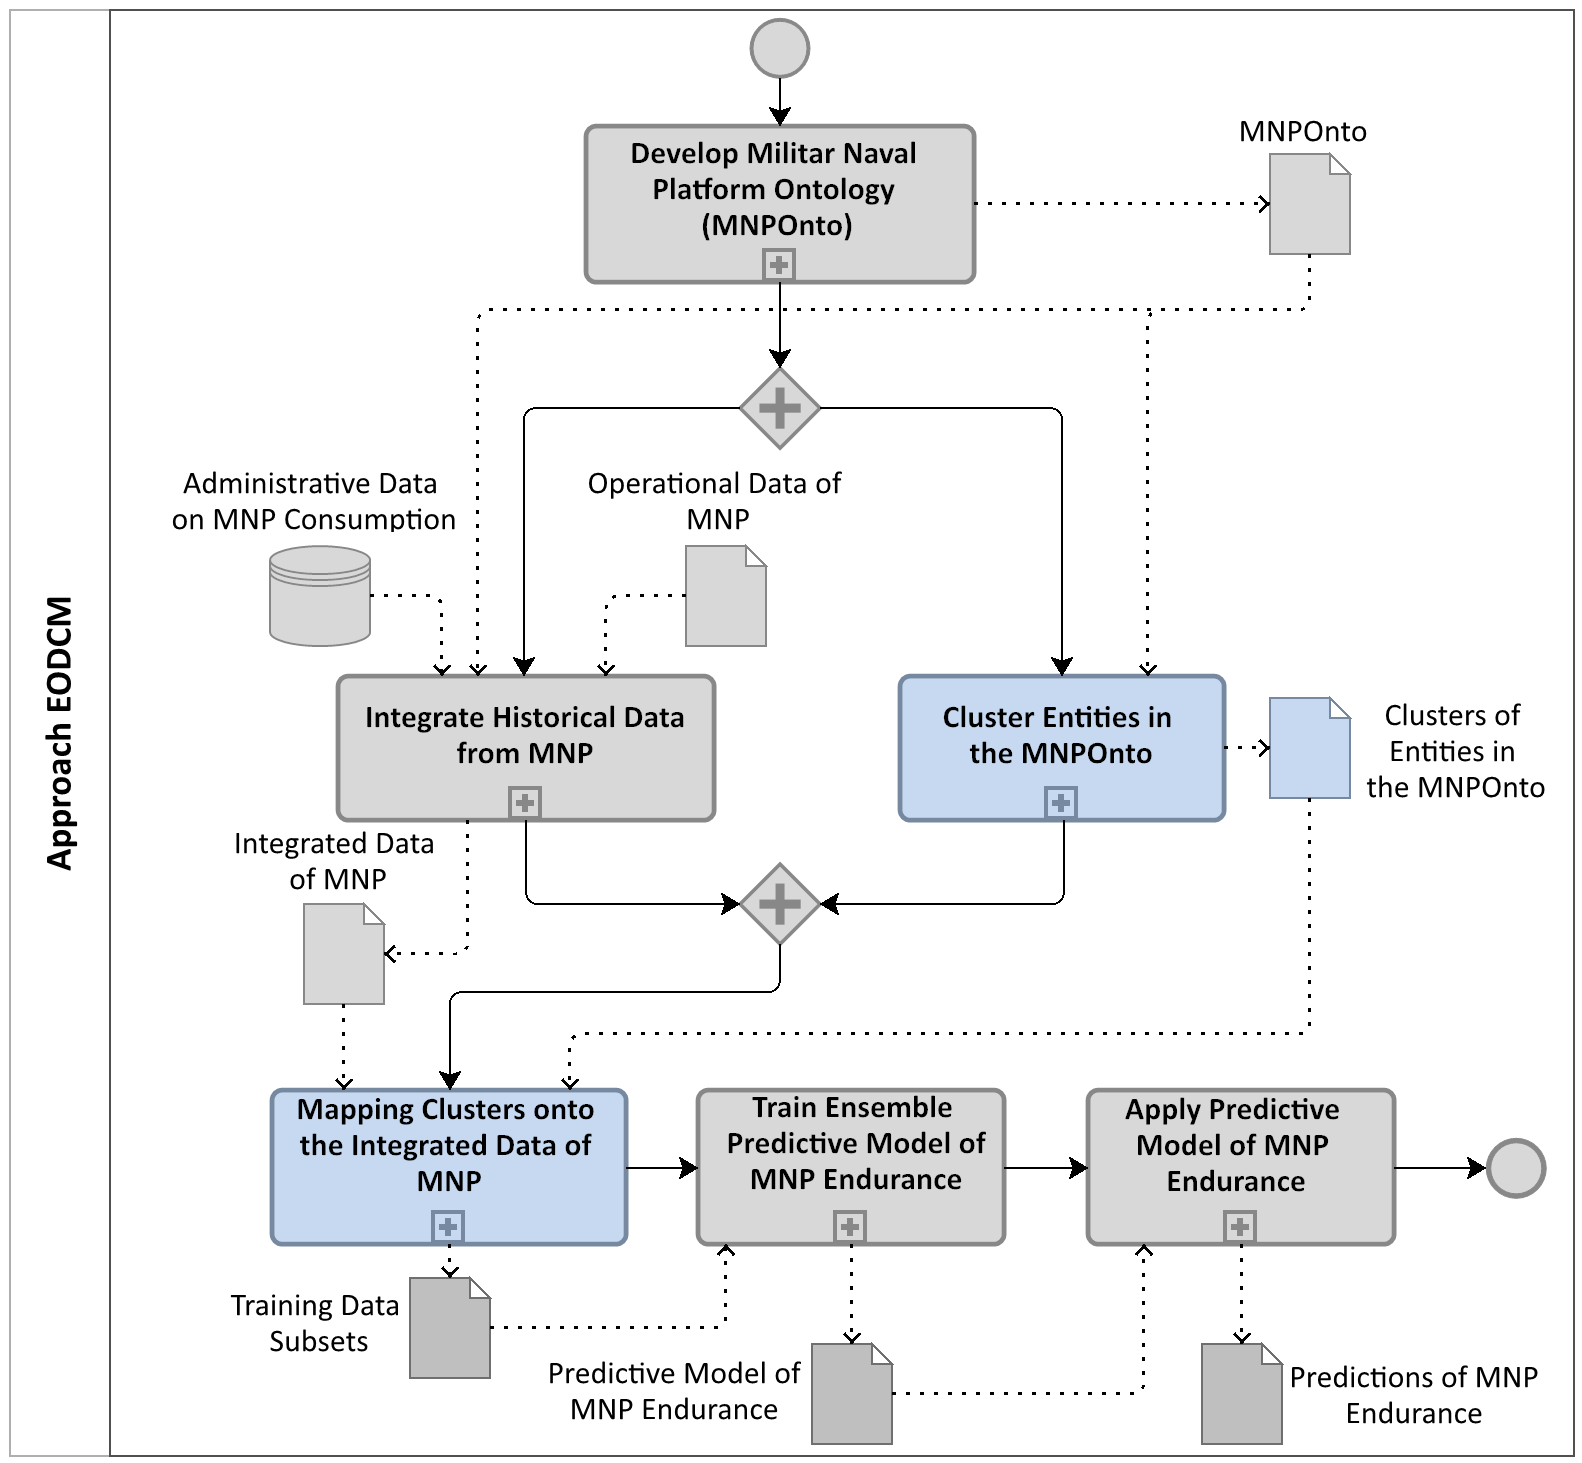
\includegraphics[width=\linewidth]{images/visao-geral-en.png}
    \caption{Overview of the EODCM approach}
    %\par \small{Overview of the EODCM approach}
    \label{fig:approach}
\end{figure}

\par A abordagem consiste em modelar o domínio com objetivo de obter um conhecimento compartilhado. Esse conhecimento poderia ser utilizado na construção do modelo preditivo.

\par De maneira resumida, o que está sendo proposto aqui é que sempre devemos modelar para predizer.

\subsection{The Military Naval Platform Ontology}

\subsection{Predictive Model Pipeline}
Construção do modelo preditivo
Trajetória de ciência de dados

%%
%% Experimentação
\section{Experiments and Results}

Experimentos:
\begin{enumerate}
\item modelos individuais sem mc;
\item modelos de comitê sem mc;
\item modelos de comitê com mc;
\end{enumerate}

Aplicação de teste de significância estatística 

The table \ref{tab:comparison-original} compares the results of the models using the metrics coefficient of determination (R²) and root mean squared error (RMSE), considering only the original data.

\begin{table*}[ht]
  \caption{Comparison of trained models on the original dataset}
  \label{tab:comparison-original}
  \begin{tabular}{ccl}
    \toprule
    Models & R² & RMSE \\
    \midrule
    Linear Regression & 0.74 & 5.14\\
    Decision Tree & 0.78 & 4.69\\
    Random Forest & 0.81 & 4.33\\
    Gradient Boosting & 0.83 & 4.13\\
    K-Nearest Neighbors & 0.29 & 8.47\\
    %Support Vector Regression & -0.10 & 10.54\\
    %Multi-Layer Perceptron & -2.59 & 19.03\\
    Ensemble without ODCM & 0.84 & 4.07\\
    \textbf{EODCM} & \textbf{0.97} & \textbf{1.87}\\
  \bottomrule
\end{tabular}
\end{table*}


Otherwise, the table \ref{tab:comparison-synthetic} compares the results of the models using datasets with the addition of synthetic data.

\begin{table*}[ht]
  \caption{Comparison of trained models on the synthetic data}
  \label{tab:comparison-synthetic}
  \begin{tabular}{ccl}
    \toprule
    Models & R² & RMSE \\
    \midrule
    Linear Regression & 0.64 & 3.84\\
    Decision Tree & 0.93 & 1.64\\
    Random Forest & 0.92 & 1.81\\
    \textbf{Gradient Boosting} & \textbf{0.96} & \textbf{1.21}\\
    K-Nearest Neighbors & 0.89 & 2.11\\
    %Support Vector Regression & -0.10 & 10.54\\
    %Multi-Layer Perceptron & -2.59 & 19.03\\
    Ensemble without ODCM & 0.95 & 1.49\\
    EODCM & 0.94 & 1.61\\
  \bottomrule
\end{tabular}
\end{table*}

%%
%% Conclusão
\section{Conclusion}

A incorporação de MC em AM foi positivamente evidenciada.

Limitações

\par Trabalhos futuros


%%
%% Agradecimentos
\section{Acknowledgments}

This research has been funded by FINEP/DCT/FAPEB (no. 2904/20-01.20.0272.00) under the S2C2 project.

%%
%% Define the bibliography file to be used
\bibliography{sample-ceur}

%%
%% If your work has an appendix, this is the place to put it.
%\appendix
%\section{Online Resources}


\end{document}

%%
%% End of file
